\chapter{Utilities}
\label{chap:util}

Currently, there are \num{15} utilities. Users can access the utilities in two ways. From the main interface (\autoref{fig:mainWindow}) users can select Utilities in the list to the right and a new window will appear with a complete list of available utilities (\autoref{fig:utilWindow}). The alternative option is to directly select the desired utility from the menu entry, Utilities. The second approach is faster since does not require to use the Utilities window.

The utilities are organized in General Utilities and utilities that are specific for a given module. The following sections describe each one of the implemented utilities.

\begin{figure}[h]
	\centering
	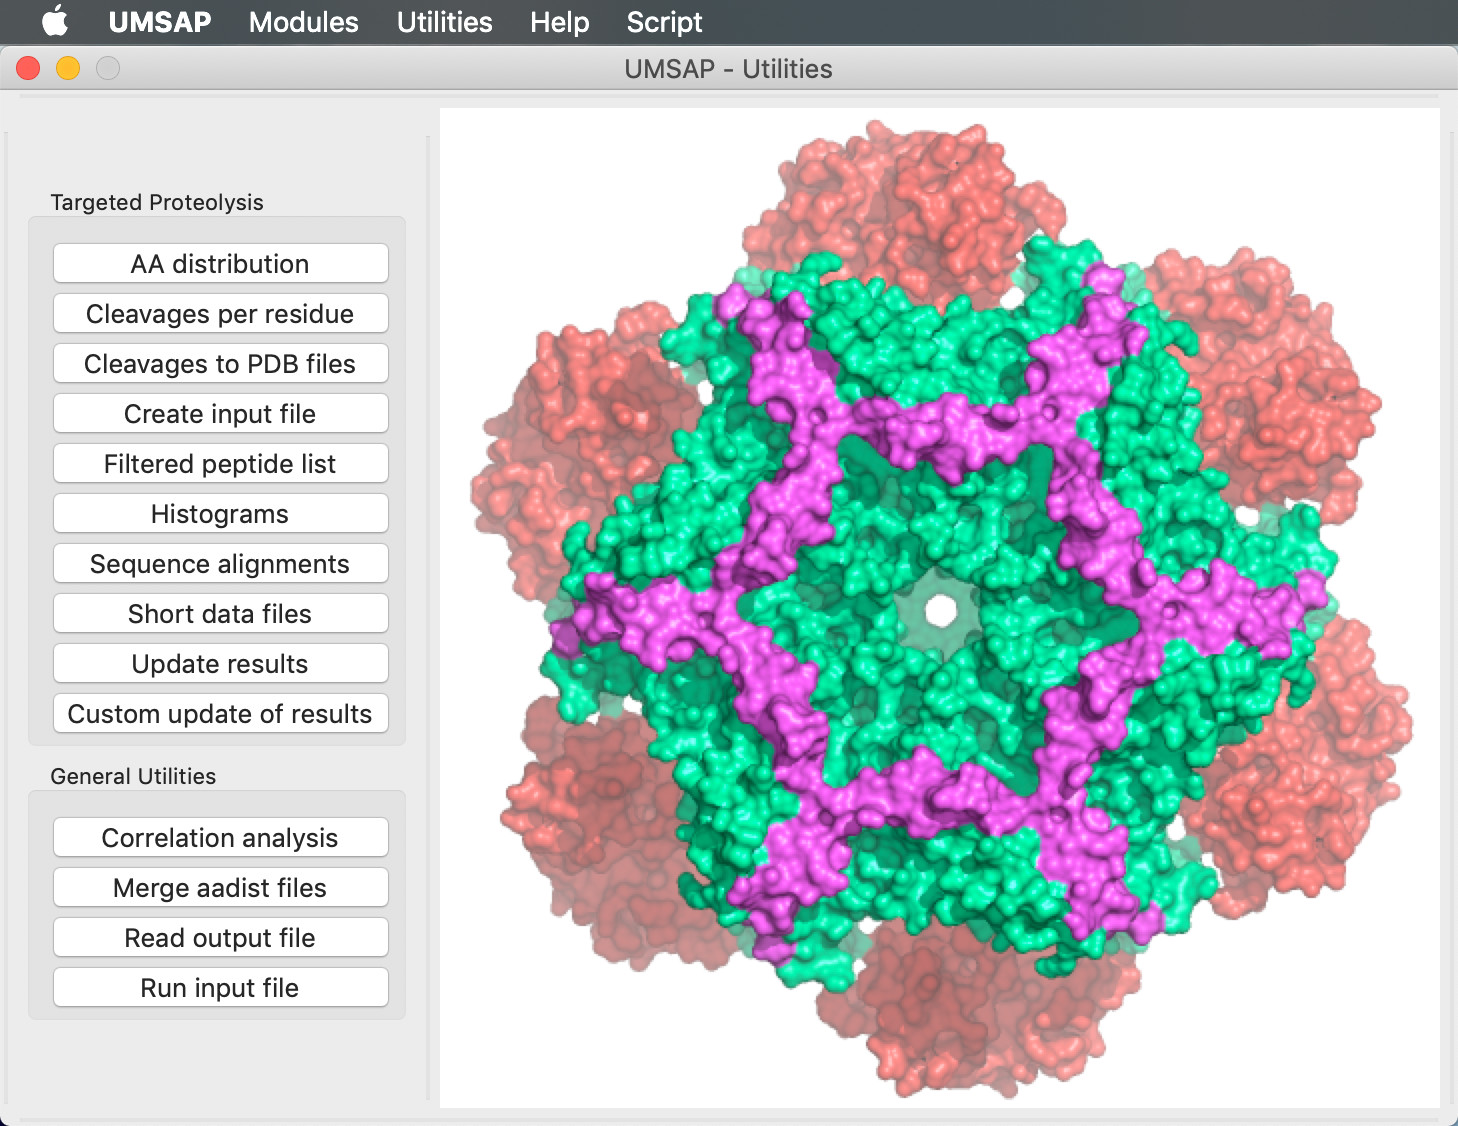
\includegraphics[width=0.7\textwidth]{./IMAGES/UTIL-WINDOW/util.jpg}	    
	\caption[The Utilities window]{\textbf{The Utilities window.} From this window users can access all the available utilities.} 
	\label{fig:utilWindow}
	\vspace{-5pt} 	
\end{figure} 

\section{Limited Proteolysis utilities}

\subsection{Sequence highlight}
\label{subsec:utilSeqHigh}
The Sequence Highlight utility allows user to highlight on the sequence of the Target protein the peptides detected in each gel lane/band considered in the .limprot file. The sequences with the highlighted peptides are saved in a .pdf file. How to generate a .limprot file is discussed in \autoref{chap:limprot}.

\textit{\textbf{The interface}}

The window of the Sequence Highlight utility is divided in three regions. 

\begin{figure}[h]
	\centering
	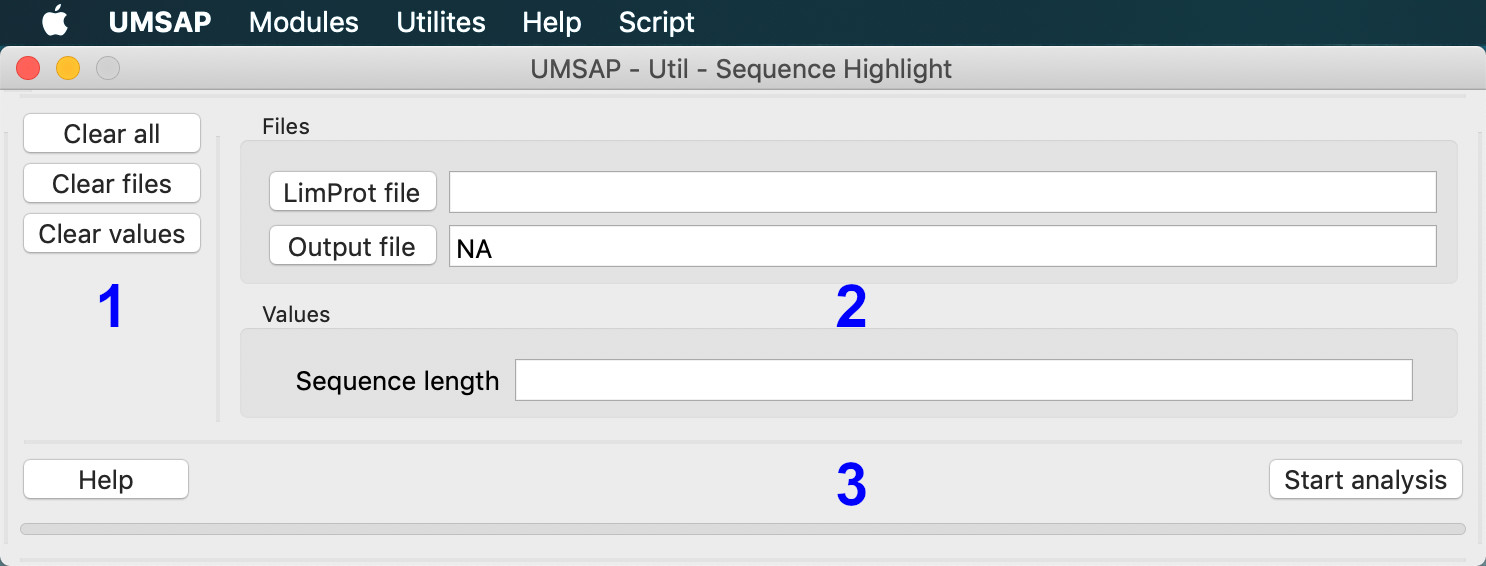
\includegraphics[width=0.7\textwidth]{./IMAGES/UTIL-SEQUENCE-HIGHLIGHT/sequence-highlight.jpg}	    
	\caption[The Sequence Highlight utility window]{\textbf{The Sequence Highlight utility window.} This window allows to generate a .pdf file showing the location of the peptides detected in the investigated gel lane/band on the sequence of the Target protein.} 
	\label{fig:seqhighwindow}
	\vspace{-5pt} 	
\end{figure} 

Region \num{1} contains three buttons allowing users to quickly delete all provided input to generate a new .pdf file. The Clear all button will delete all user provided input. The Clear files button will delete the path to all user provided files. Finally, the Clear values button will delete all user provided numerical values.

Region \num{2} contains the fields where users provide the information needed in order to create the .pdf file with the highlighted sequences. The Limprot file button allows users to browse the file system to select the .limprot file that will be used for the generation of the .pdf file. Only one .limprot file can be provided here. The Output file button allows users to browse the file system to select the location and name of the .pdf file. If left empty, then the .pdf file, resulting from the analysis, will be saved in the same directory containing the .limprot file and will have the same name as the .limprot file. If the folder containing the selected .limprot file already contains a .pdf file with the same name as the selected .limprot file, then UMSAP will add the current date and time to the second to the end of the .pdf file name in order to avoid overwriting the older .pdf file without explicit user permission.

The Sequence length parameter allows user to define the maximum number of residues per line to be used during the creation of the .pdf file. The value here must be an integer number greater than zero.

Region \num{3} contains the Help and Start analysis buttons and a progress bar. The Help button leads to an online tutorial while the Start analysis button will start the generation of the .pdf file. The progress bar will give users a rough idea of the remaining processing time once the analysis is started.

\textit{\textbf{The analysis}}

First, UMSAP will check the validity of the user provided input. After this, for each gel lane/band analyzed in the .limprot file, UMSAP will print the sequence of the Target protein to the .pdf file with the peptides found in the gel lane/band highlighted in red.

\textit{\textbf{The output}} 

The output is a .pdf file containing a page for each gel lane/band found in the .limprot file. As described before, each page contains the sequence of the Target protein with the detected peptides highlighted in red. In addition, the residue number of the beginning and ending of the highlighted fragments are also given. If the sequence of the native protein was provided when creating the .limprot file, then the information is given for the recombinant and native protein. 

\textit{\textbf{The Tools menu}}

This utility does not have a Tool menu.

\section{Targeted Proteolysis utilities }  

\subsection{AA Distribution}
\label{subsec:utilAadistCalc}
The AA Distribution utility allows user to calculate the AA distribution around the detected cleavage sites using a list of FP (see page \pageref{par:tarprotPIP}). The list of FP is automatically generated from a .tarprot file. How to generate a .tarprot file is discussed in \autoref{chap:tarprot}. The list of FP is a non redundant list. 

\textit{\textbf{The interface}}

The window of the AA Distribution utility is divided in three regions (\autoref{fig:utilAadistCalc}).

\begin{figure}[h]
	\centering
	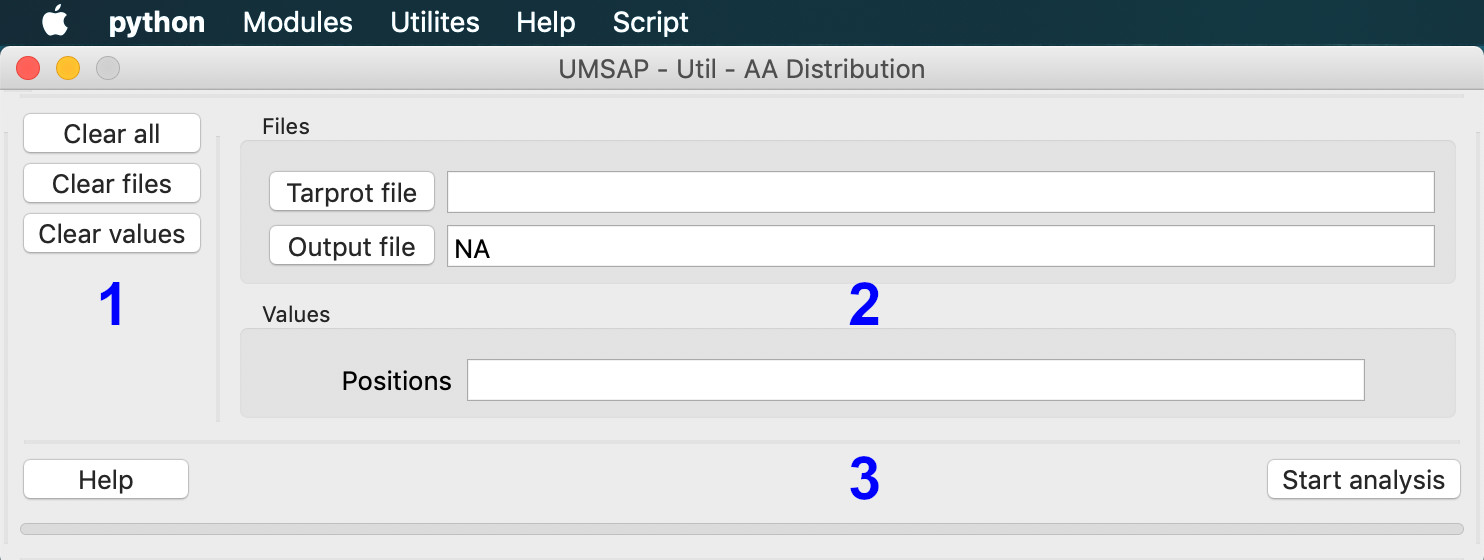
\includegraphics[width=0.7\textwidth]{./IMAGES/UTIL-AA-WINDOW/util-aa.jpg}	    
	\caption[The AA Distribution utility window]{\textbf{The AA Distribution utility window.} This window allows to obtain the AA distribution around the detected cleavage sites from a .tarprot file.} 
	\label{fig:utilAadistCalc}
	\vspace{-5pt} 	
\end{figure}

Region \num{1} contains three buttons allowing users to quickly delete all provided input and start a new distribution analysis. The Clear all button will delete all user provided input. The Clear files button will delete the path to all user provided files. Finally, the Clear values button will delete all user provided numerical values.

Region \num{2} contains the fields where users provide the information needed in order to perform the AA distribution calculation. The Tarprot file button allows users to browse the file system to select the .tarprot file that will be used for the analysis. Only one .tarprot file can be provided here. The Output file button allows users to browse the file system to select the location and name of the Output file. If left empty, then the .aadist file, resulting from the analysis, will be saved in the same directory containing the .tarprot file and will have the same name as the .tarprot file. If the folder containing the selected .tarprot file already contains a .aadist file with the same name as the selected .tarprot file, then UMSAP will add the current date and time to the seconds to the end of the .aadist file in order to avoid overwriting the older .aadist file without explicit user permission.    

The parameter Positions indicates the number of positions around the cleavage sites to be analyzed. The value here must be an integer number greater than zero.

Region \num{3} contains the Help and Start analysis buttons and a progress bar. The Help button leads to an online tutorial while the Start analysis button will start the analysis. The progress bar will give users a rough idea of the remaining processing time once the analysis is started.

\textit{\textbf{The analysis}}

First, UMSAP will check the validity of the user provided input. After this, a list of FP is created using the .tarprot file. For each FP, the sequence around the N and C terminal ends of the peptide is analyzed up to the user provided number of Positions. For the N terminus of the peptide the identity of residues in positions \(Pn\) to \(P1\) is inferred from the sequence of the recombinant protein contained in the .tarprot file. The same is done for positions \(P1'\) to \(Pn'\) at the C terminus of the peptide. If the N or C terminus of a peptide is the first or last residue of the recombinant protein under study the N or C terminus is excluded from the analysis. For each position the number of times that each AA appears at a given position are counted. Finally, the absolute numbers of AA appearances for each position are converted to percent taking the total for each position as the sum of all counted AA in the position.

In addition, UMSAP tests whether the obtained AA distribution is significantly different to the expected AA distribution from the proteolysis of the Target protein by a totally non-selective protease. The first step is to generate an AA distribution with the same number of positions defined by the user with the Position parameter. This distribution is generated assuming that all peptidic bonds in the recombinant protein may be cleaved by the protease with equal probability and that all peptidic bonds will be cleaved. Here, we are also assuming that all products of cleaving all peptidic bonds will be detected in the MS experiment. Then, UMSAP compares each position in both distributions using a $\chi^2$ test with the significance level found in the .tarprot file. In order to be able to perform the $\chi^2$ test, AAs are pooled together in the same groups as described below for the color code used in the output.    

\begin{figure}[h]
	\centering
	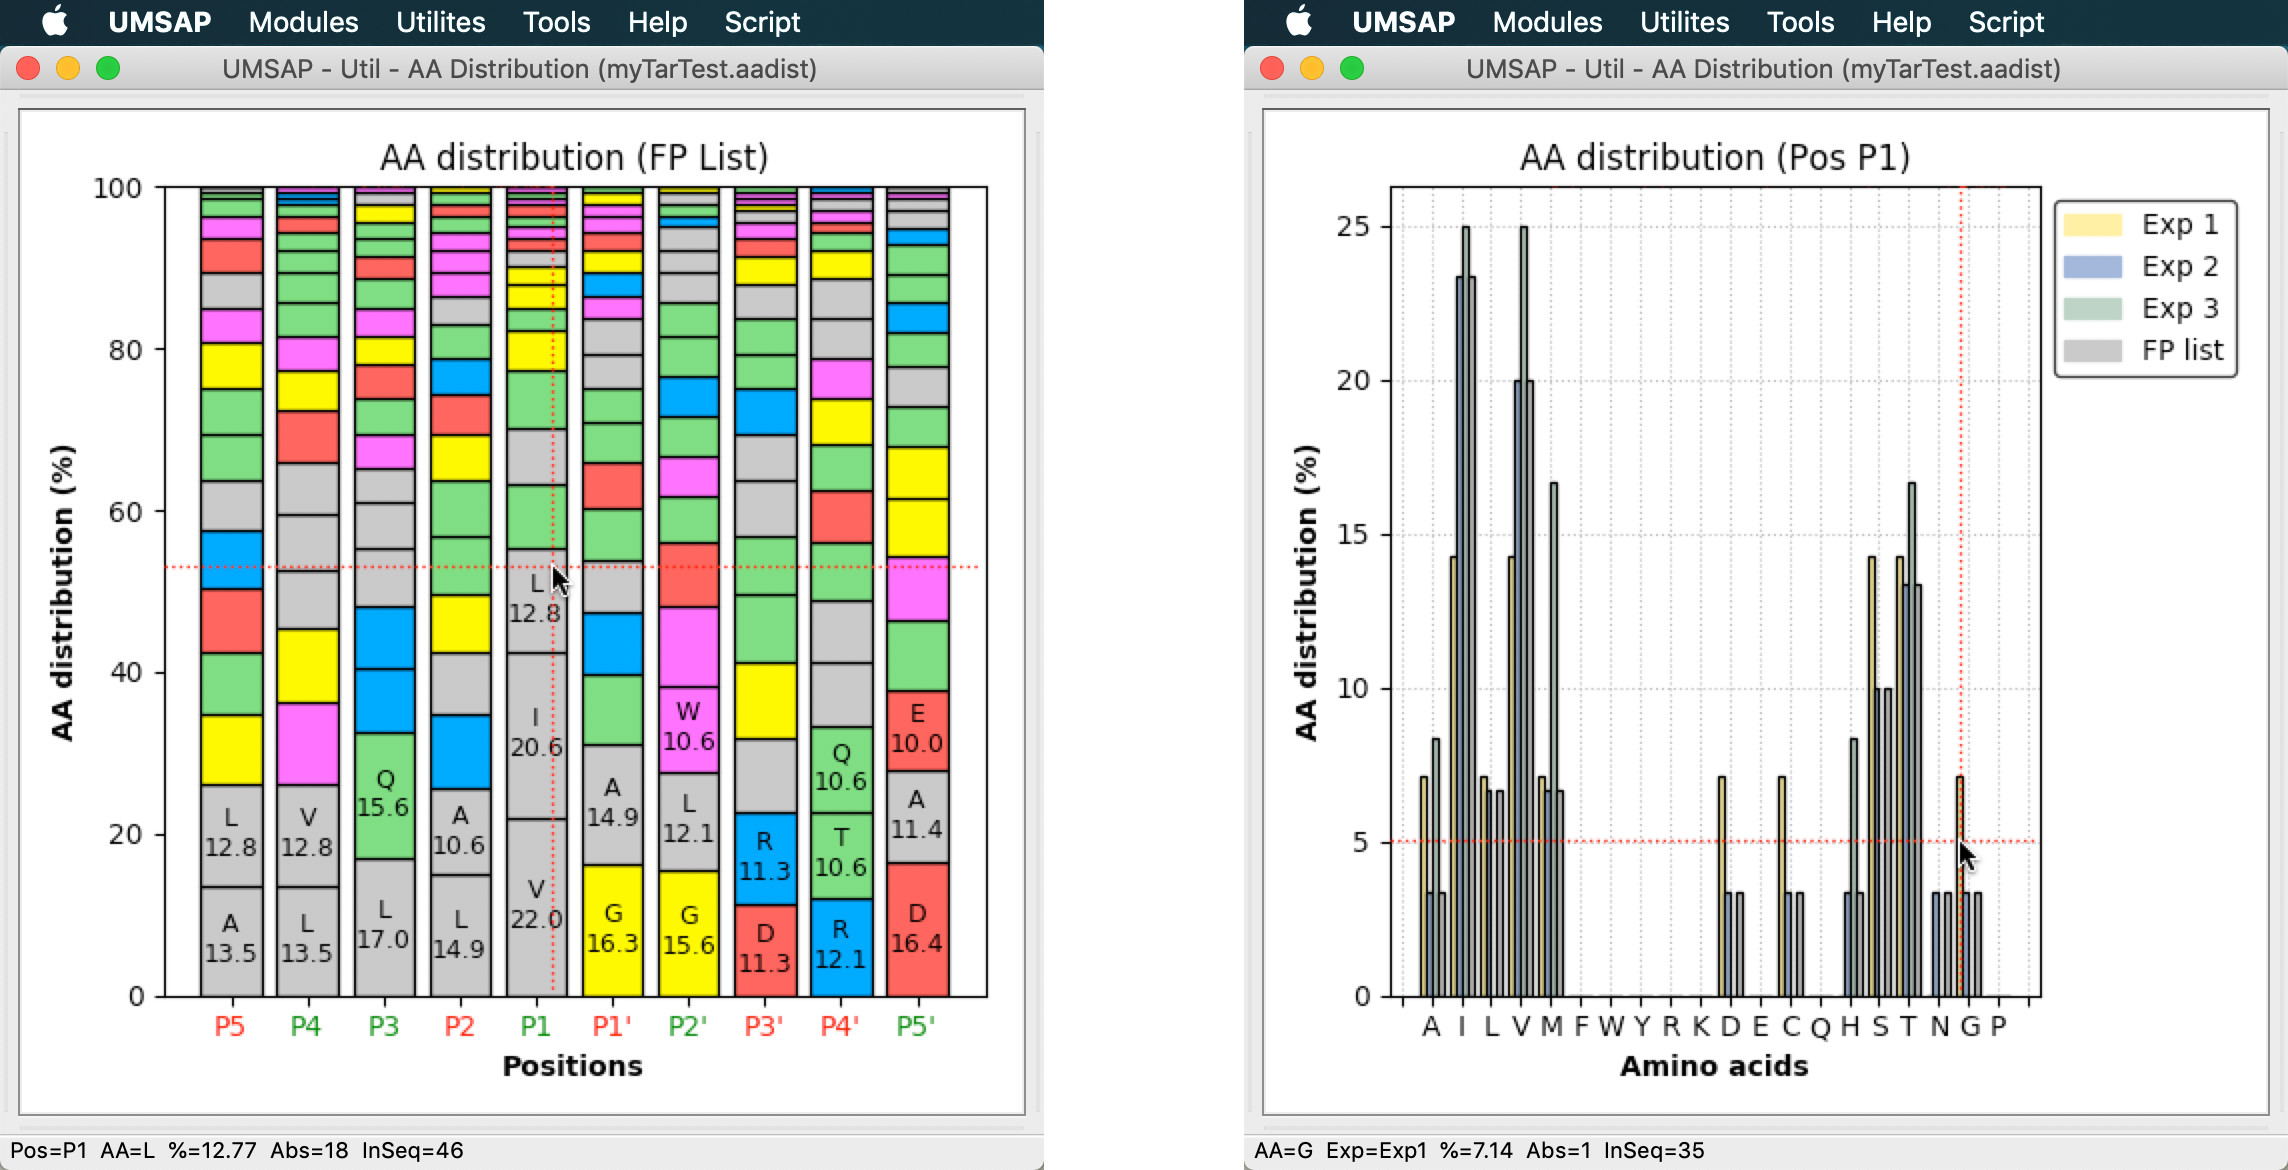
\includegraphics[width=0.9\textwidth]{./IMAGES/UTIL-AA-WINDOW/util-aa-res.jpg}	    
	\caption[The AA Distribution analysis window]{\textbf{The AA Distribution analysis window.} This window allows to visualize the results contained in a .aadist file.}
	\label{fig:utilAadistShow}
	\vspace{-5pt} 	
\end{figure}

\textit{\textbf{The output}} 

The output from the AA distribution calculation is a file with .aadist extension. The file will be automatically loaded and a graphical representation of the results will be shown (\autoref{fig:utilAadistShow}). There are two graphical representations. The first representation shows a bar graph of the AA distribution in which each bar represents a position. AAs are color coded with positively charged AAs (R and K) in blue, negatively charged AAs (D and E) in red, polar AAs (S, T, N, H, C and Q) in green, non-polar AAs (A, V, I, L and M) in gray, aromatic AAs (F, Y and W) in pink and Gly and Pro in yellow. AAs with an occurrence higher than \SI{10}{\percent} are labeled with the one letter code for the AA and the percentage value. For example, in \autoref{fig:utilAadistShow} the value of \SI{16.7}{\percent} obtained for A in position \(P1'\) means that A was found in position \(P1'\) in the \SI{16.7}{\percent} of the total cleavage sites detected. 

The results of the $\chi^2$ test are given in the color of the name of the position. A green color represents that the obtained distribution in the position is significantly different to a no selectivity distribution at the level of significance found in the .tarprot file. A red color represents that the distributions are not significantly different at the level of significance found in the .tarprot file. Finally, a black color indicates that the number of expected values below 5 was higher than the \SI{20}{\percent} threshold recommended by Yates et al. and the test was not performed \cite{Yates1999}. 

If the mouse pointer is placed on top of the bars, then information related to the bar and the AA will be shown in the status bar at the bottom of the window. The information includes the Position (Pos), the amino acid (AA), how many times does the AA appears in the position as a percent of the total AA count for the given position (\%) and the absolute number (Abs) and how many times does the AA appears in the sequence of the recombinant protein (InSeq).

The second representation allows to compare the AA distribution in one position across all experiments. This is also a bar representation in which each bar represents an experiment and each position an AA. Placing the mouse pointer over a bar shows information about it. The information includes the AA (AA), the experiment (Exp), how many times does the AA appears in the position for the given experiment as a percent of the total AA count found at the position for the given experiment (\%) and  the absolute number (Abs) and how many times does the AA appears in the sequence of the recombinant protein (InSeq).

\textit{\textbf{The Tools menu}}

By default, the AA distribution for all AA in the FP list will be shown when the .aadist file is loaded. The Tools menu in the window allows user to change the displayed experiment or to select the position for which results in the experiments should be compared. In addition, users may select to save a figure of the plot and to reset the view. 

\subsection{Cleavages per Residue}
\label{subsec:utilCutsPerRes}
The Cleavages per residue utility calculates the absolute number of cleavages detected in the MS experiments for each residue in the recombinant protein under study. The peptides used to identify the cleavage sites are the FP contained in the .tarprot file used as input for the calculation (see page \pageref{par:tarprotPIP}). How to generate the .tarprot file is discussed in \autoref{chap:tarprot}. The FP list is a non redundant list.

\textit{\textbf{The interface}}

The Cleavages per residue utility does not have a window since there are no options to specify. When the utility is selected users will be asked to select a .tarprot file and then users must select the output file. That is all.

\textit{\textbf{The analysis}}

First, UMSAP will check the validity of the user provided input. After this the list of FP will be generated from the .tarprot file. Then, UMSAP will count how many times each residue in the protein under study appears at the C terminus of a FP or at the \(N-1\) position of a FP (\(N\) is the N terminus of the FP). The cleavages per residue value for the first and last residue of the protein under study is of course zero. This is done for every experiment in the .tarprot file and also taking into account the results for all experiments. Finally, UMSAP will take the absolute number of cleavages per residue and will normalize the values to bring them in the 0 to 1 range. Both the absolute and normalized values are written to the output file. After the analysis is done the results will be automatically loaded and displayed in a new window (\autoref{fig:utilCutsPerRes}). 

\textit{\textbf{The output}}

The output file from the Cleavages per residue utility will be shown as a simple number of cleavages vs residue number plot (\autoref{fig:utilCutsPerRes}). Residues with cleavages per residue higher than one third of the maximum number of cleavages per residue will be highlighted with an asterisk (*). Placing the mouse pointer inside the plot will display the residue number and the number of cleavages in the status bar at the bottom of the window. When two data sets are plotted simultaneously, the number of cleavages are given in the same order shown by the legend in the window. The gray vertical lines enclose the native residues. 

\textit{\textbf{The Tools menu}}

The window shows by default the absolute number of cleavages considering all FP for the recombinant protein. The Tools menu allows users to change this. Users may select to plot the results for a particular experiment or to compare two experiments. In addition, only the native sequence could be plotted or the normalized cleavages per residue values may be shown. An image of the plot can be created using the Save Plot Image entry in the Tools menu. The Reset View option restores the default appearance of the window.   

\begin{figure}[h]
	\centering
	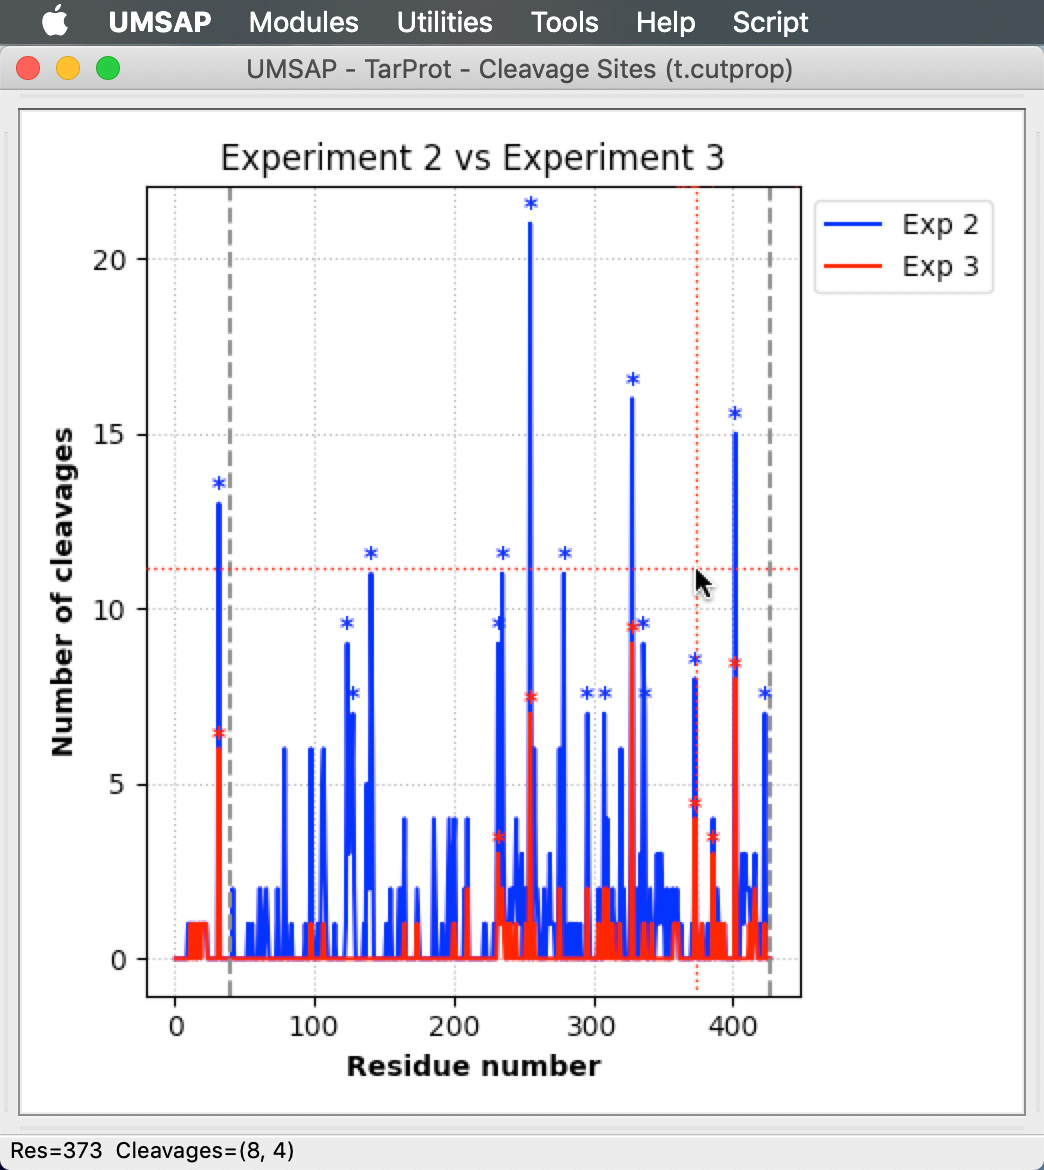
\includegraphics[width=0.7\textwidth]{./IMAGES/UTIL-CUTPROP-WINDOW/util-cutprop-res.jpg}	    
	\caption[The Cleavages per Residue analysis window]{\textbf{The Cleavages per Residue analysis window.} This window allows to visualize the results contained in a .cutprop file.} 
	\label{fig:utilCutsPerRes}
	\vspace{-5pt} 	
\end{figure}

\subsection{Cleavages to PDB Files}
\label{subsec:utilCut2Pdb}

The Cleavages to PDB Files utility maps the number of cleavages per residue found in a .tarprot file to a .pdb file containing the structure of the Target protein. The peptides used to identify the cleavage sites are the FP contained in the .tarprot file used as input for the calculation, see page \pageref{par:tarprotPIP}. How to generate the .tarprot file is discussed in \autoref{chap:tarprot}. The FP list is a non redundant list.

\textit{\textbf{The interface}}

The Cleavages to PDB Files window is divided in three regions, see \autoref{fig:utilCut2PDB}.

Region \num{1} contains three buttons allowing users to quickly delete all provided input and start a new distribution analysis. The Clear all button will delete all user provided input. The Clear files button will delete the path to all user provided files. Finally, the Clear values button will delete all user provided numerical values.

Region \num{2} contains the fields where users provide the information needed in order to perform the mapping of the number of cleavages. The Tarprot file button allows users to browse the file system to select the .tarprot file that will be use for the analysis. Only one .tarprot file can be provided here. The PDB file allows user to browse the file system to select a .pdb file. The .pdb file will contain the structure of the Target protein. This field can be left empty if the PDB file is to be downloaded from the PDB database. The Output folder button allows users to browse the file system to select the location of the resulting PDB folder containing the results. If left empty, then the PDB folder, resulting from the analysis, will be saved in the same directory containing the .tarprot file. If the Output folder option is left empty and the folder containing the selected .tarprot file already contains a PDB folder, then UMSAP will add the current date and time to the second to the end of the folder name in order to avoid overwriting the older PDB folder without explicit user permission.

The PDB ID field allows users to specify the chain or the segment id in the .pdb file that should be used for the mapping. Alternatively, if the PDB file field is left empty a code from the PDB database plus the chain or segment id may be given here. In this case, the pdb file will be directly downloaded from the PDB database. The expected syntax in this case is code:chain or code:segment for example, 2f4y:A or 2f4y:PROA.  

Region \num{3} contains the Help and Start analysis buttons and a progress bar. The Help button leads to an online tutorial while the Start analysis button will start the analysis. The progress bar will give users a rough idea of the remaining processing time once the analysis is started.

\begin{figure}[h]
	\centering
	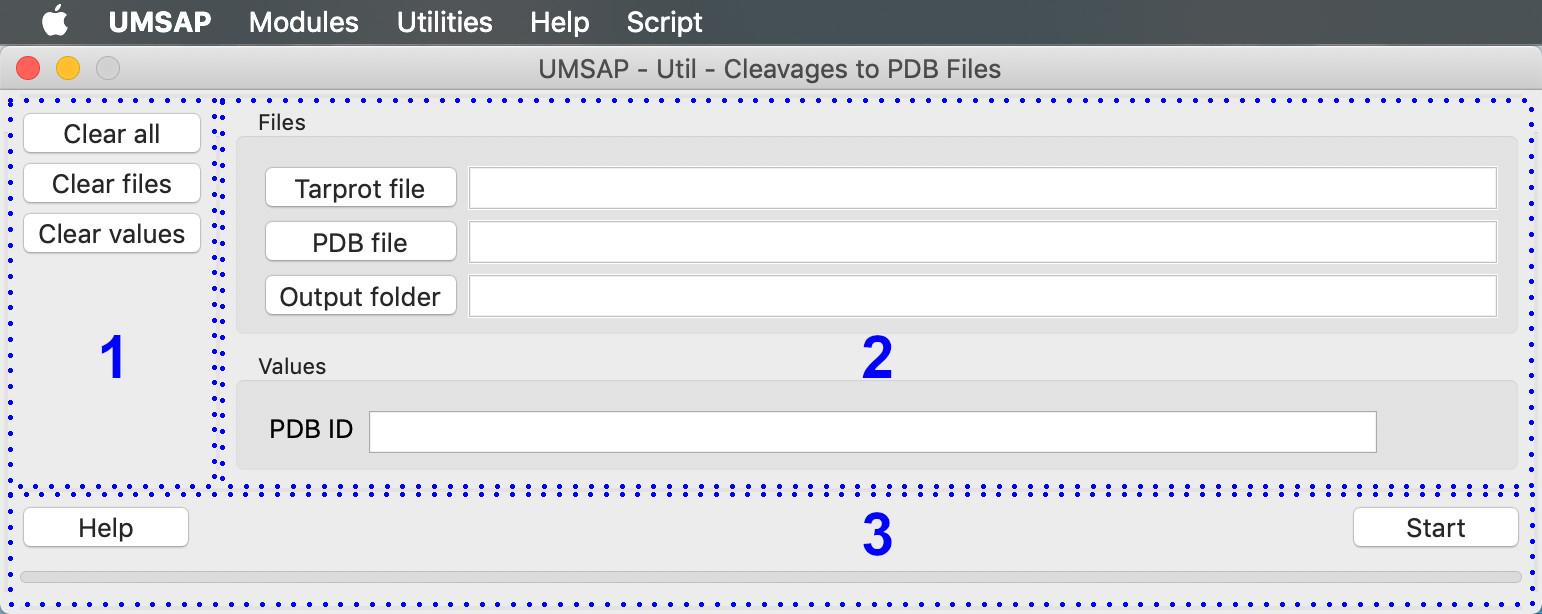
\includegraphics[width=0.7\textwidth]{./IMAGES/UTIL-PDB-WINDOW/util-pdb.jpg}	    
	\caption[The Cleavages to PDB Files utility window]{\textbf{The Cleavages to PDB Files utility window.} This window allows to map the detected number of cleavages per residue to a .pdb file containing the structure of the Target protein. The number of cleavages are mapped to the beta field in the .pdb.} 
	\label{fig:utilCut2PDB}
	\vspace{-5pt} 	
\end{figure}

\textit{\textbf{The analysis}}

First, UMSAP will check the validity of the user provided input. Then, a temporal .cutprop file will be created. Details about the .cutprop files can be found in \autoref{subsec:utilCutsPerRes}. After this, the sequence from the .pdb file is extracted and aligned with the sequence of the recombinant protein found in the .tarprot file. Finally, the number of cleavages found in the .cutprop file are mapped to the corresponding residues in the .pdb file.

\textit{\textbf{The output}}

The output from this utility is a series of .pdb files that will be saved in a PDB folder. Each file contains the number of cleavages mapped to the beta field of the corresponding residue in the .pdb structure. The results for each experiment and the FP list are mapped to individual files. The mapped values can be visualized by opening the .pdb files with VMD, PyMol or Chimera and coloring the structure by beta factors.

\subsection{Filtered Peptide List}
\label{subsec:utilFiltPept}

The Filtered Peptide List utility allows users to read a .tarprot file and to create a .filtpept file containing the FP list. How to generate the .tarprot file is discussed in \autoref{chap:tarprot}. The FP list is a non redundant list of all peptides identified during the Targeted Proteolysis analysis.

\textit{\textbf{The interface}}

The Filtered Peptide List utility does not have a window since there are no options to specify. When the utility is selected users will be asked to select a .tarprot file and then users must select the output file. That is all.

\textit{\textbf{The analysis}}

First, UMSAP will check the validity of the user provided input. Then the .tarprot file will be read in and all FP will be saved to the output file.

\textit{\textbf{The output}}

The .filtpept file has a tabular format in which the first row contains the name of the columns and columns are tab separated. It is a plain text file that can be read with any text editor. The file list all filtered peptides indicating the first and last residue number of the peptides and in which experiments were the peptide detected. A value of 1 in the experiment columns indicates that the peptide has intensity values that are significantly different to the control at the chosen significance level. A value of 0 indicates otherwise.

\subsection{Histograms}
\label{subsec:utilHistoCut}
The Histograms utility allows to create histograms of the identified cleavage sites using the residue numbers of the Target protein as the definition of the windows in the histograms. Histograms are created from a .tarprot file. How to generate the .tarprot file is discussed in \autoref{chap:tarprot}. Only FP are used to create the histograms, see page \pageref{par:tarprotPIP}. The list of FP is a non redundant list. 

\textit{\textbf{The interface}}

The Histograms window is divided in three regions (\autoref{fig:utilHistoCut}).

\begin{figure}[h]
	\centering
	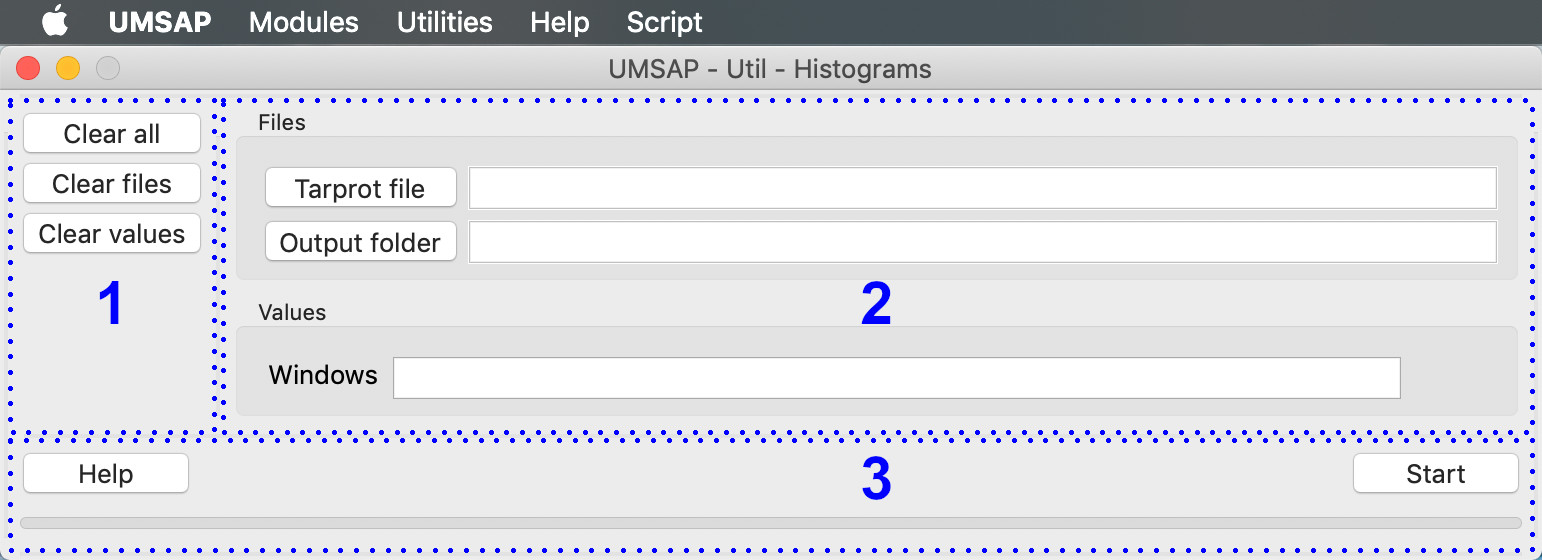
\includegraphics[width=0.9\textwidth]{./IMAGES/UTIL-HIST-WINDOW/util-histo.jpg}	    
	\caption[The Histograms utility window]{\textbf{The Histograms utility window.} This window allows to create histograms of the identified cleavage sites using the residue numbers of the Target protein as the definition of the windows in the histograms.} 
	\label{fig:utilHistoCut}
	\vspace{-5pt} 	
\end{figure}

Region \num{1} contains three buttons allowing users to quickly delete all provided input and start a new calculation. The Clear all button will delete all user provided input. The Clear files button will delete the path to all user provided files. Finally, the Clear values button will delete all user provided numerical values.

Region \num{2} contains the fields where users provide the information needed in order to create the histograms. The Tarprot file button allows users to browse the file system to select the .tarprot file that will be used for the analysis. Only one .tarprot file can be selected here. The Output file button allows users to browse the file system to select the location of the .hist file to be created. If no Output file is selected the .hist file will be created in the same directory as the selected .tarprot file. If an older .hist file exists in the selected folder, UMSAP will append the date and time to the second to the end of the .hist file name in order to avoid overwriting the old .hist file. 

The parameter Windows allows to define the length of the windows in the histograms. Values here are expected to be integers greater than zero. A single value will results in equally spaced windows covering the entire length of the recombinant protein under study. Several values will result in custom sized windows. This may be useful if users want to define windows matching a structure related property of the Target protein e.g. secondary structure. In this case, the values must be space separated and organized from lower to higher values. For example, the input \numlist{1 50 100 200 220} will create four windows covering residues \numrange{1}{49}, \numrange{50}{99}, \numrange{100}{199} and \numrange{200}{219}.

Region \num{3} contains the Help and Start analysis buttons and a progress bar. The Help button leads to an online tutorial while the Start analysis button will start the analysis. The progress bar will give users a rough idea of the remaining processing time once the analysis is started.

\textit{\textbf{The analysis}}

First, UMSAP will check the validity of the user provided input. After this, the windows of the histograms will be created and for each experiment in the .tarprot file the detected cleavage sites will be assigned to the corresponding windows. Cleavage sites are only counted once per experiment, independently of how many peptides share the same cleavage site. In addition, the total number of cleavage sites identified considering the results of all experiments is also calculated. Since most of the time the protein under study is a recombinant protein containing purification tags or only a region of the native protein, histograms are created for the residue numbers in the recombinant protein and for the residue numbers in the native protein. For this to be possible the sequence of the native protein must have been provided during the creation of the .tarprot file. In the last case cleavage sites outside the native sequence contained in the recombinant protein are discarded and the residue numbers used for the definition of the windows and cleavages sites are the residue numbers of the native sequence. After the analysis is done the .hist file will be automatically loaded and the results shown in a new window (\autoref{fig:utilHistoCutShow}).

\textit{\textbf{The output}}

The Histograms analysis window will display the results contained in a .hist file, see \autoref{fig:utilHistoCutShow}. In the histogram, experiments are shown in the order specified when creating the .tarprot file. In addition, the values for the histograms considering the results from all experiments (all FP) will be displayed as the last bar and colored in gray. Placing the mouse over the plot will display information at the bottom of the window. The information displayed includes the selected window (Win), the experiment represented by the bar (Exp) and the number of cleavages (Cleavages).

\begin{figure}[h]
	\centering
	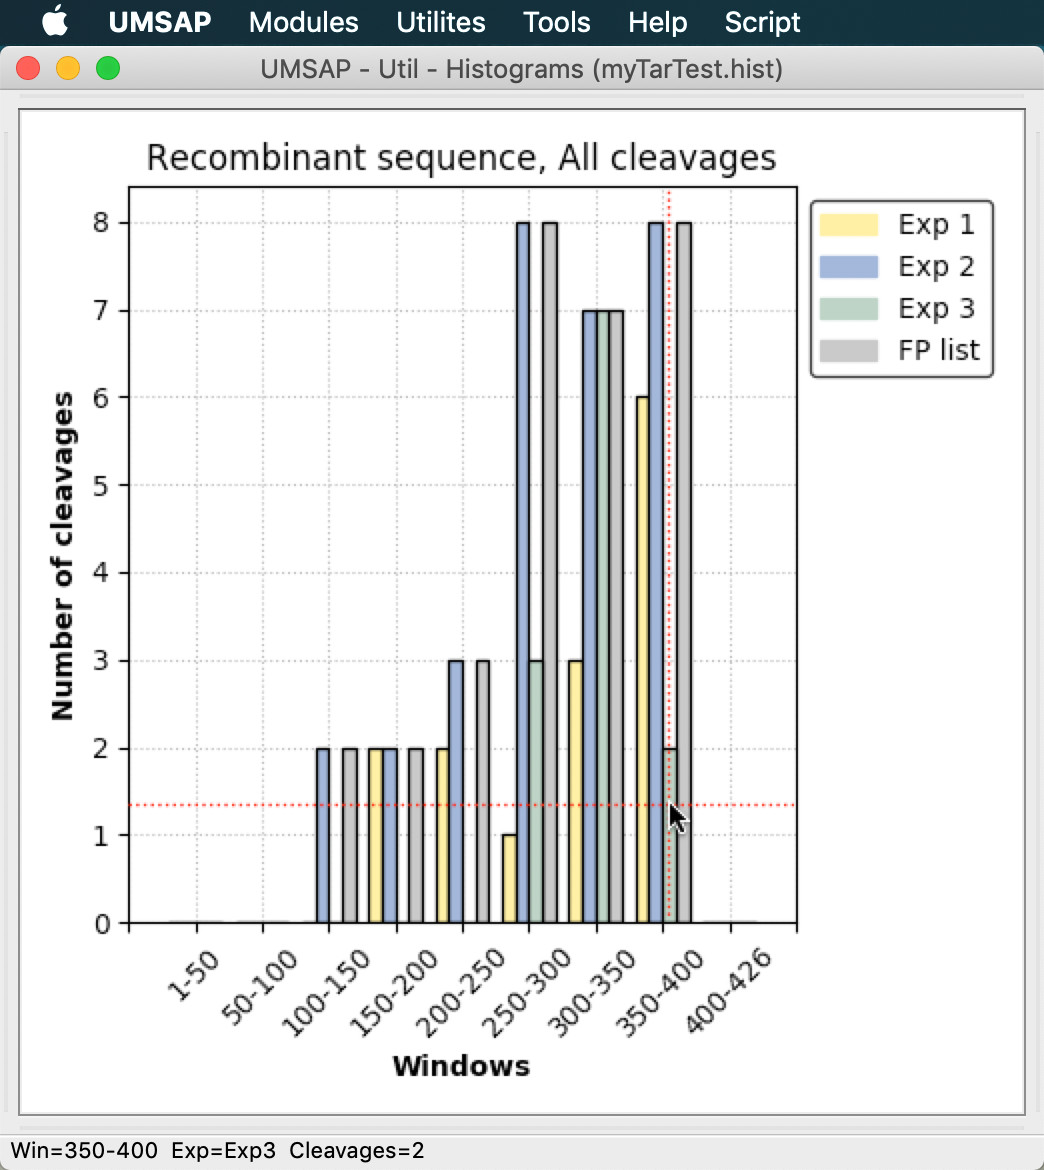
\includegraphics[width=0.7\textwidth]{./IMAGES/UTIL-HIST-WINDOW/util-histo-res.jpg}	    
	\caption[The Histograms analysis window]{\textbf{The Histograms analysis window.} This window allows to visualize the results contained in a .hist file.} 
	\label{fig:utilHistoCutShow}
	\vspace{-5pt} 	
\end{figure}

\textit{\textbf{The Tools menu}}

The Tools menu allows to show the results for the recombinant or native sequence and to show only unique cleavages or the total count of the detected cleavages. In addition, users may save an image of the plot or reset the state of the plot.

\subsection{Sequence Alignments}
\label{subsec:utilSeqAli}
The Sequence Alignments utility generates sequence alignments between the FP for each experiment and the sequence of the recombinant protein. The list of FP is generated from a .tarprot file, see page \pageref{par:tarprotPIP}. The list of FP is a non redundant list. How to generate the .tarprot file is discussed in \autoref{chap:tarprot}.

\textit{\textbf{The interface}}

The Sequence Alignments window is divided in three regions, see \autoref{fig:utilSeqAli}.

Region \num{1} contains three buttons allowing user to quickly delete all provided input and start a new calculation. The Clear all button will delete all user provided input. The Clear files button will delete the path to all user provided files. Finally, the Clear values button will delete all user provided numerical values.

Region \num{2} contains the fields where users provide the information needed in order to generate the alignments. The Tarprot file button allows users to browse the file system to select the .tarprot file that will be used for the analysis. Only one .tarprot file can be provided here. The Sequence alignments utility generates multiple files that will be saved in a folder named Sequences. The Output folder button allows users to browse the file system to select a location for the output folder Sequences. If the Output folder option is left empty, the output folder Sequences will be created in the same directory as the .tarprot file. If there is a Sequence folder in the selected Output folder, then UMSAP will create a new Sequences folder with the date and time to the second added to the end of the name in order to avoid overwriting any file. 

\begin{figure}[h]
	\centering
	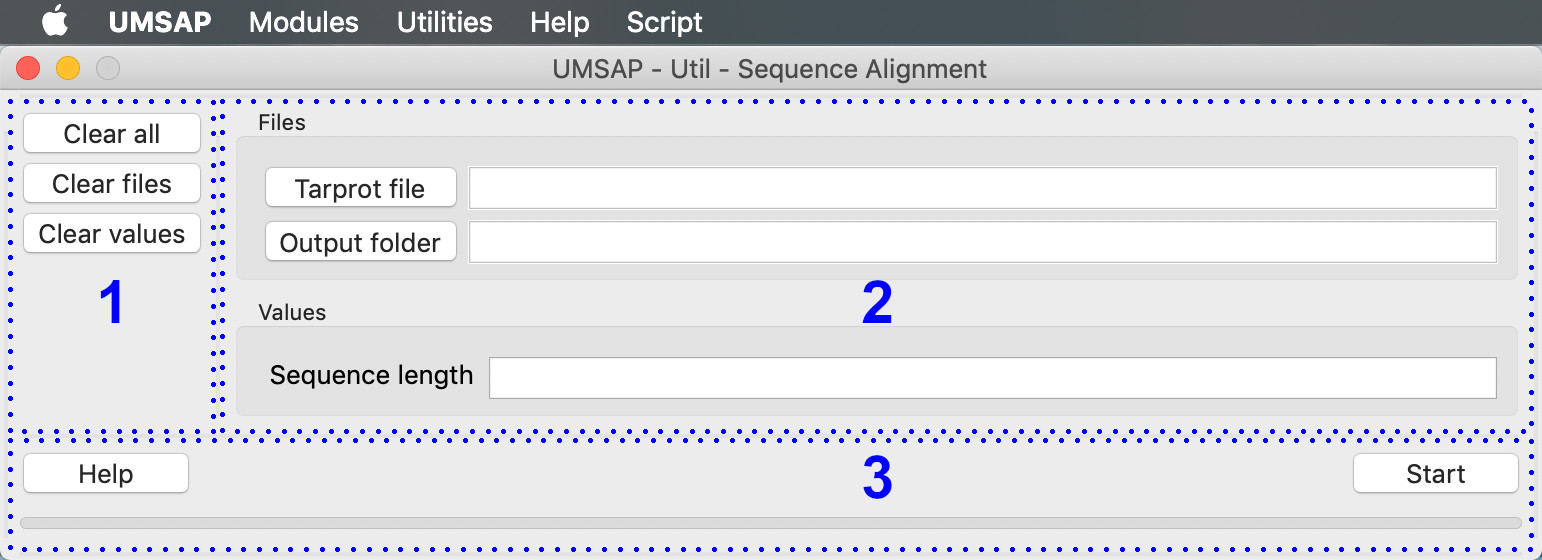
\includegraphics[width=0.7\textwidth]{./IMAGES/UTIL-SEQ-WINDOW/util-seq.jpg}	    
	\caption[The Sequence Alignments utility window]{\textbf{The Sequence Alignments utility window.} This window allows to generate sequence alignment files between the FP of each experiment and the sequence of the recombinant protein under study.} 
	\label{fig:utilSeqAli}
	\vspace{-5pt} 	
\end{figure} 

The parameter Sequence length allows to define the maximum number of residues per line in the short version of the sequence alignment files. The value here is expected to be an integer greater than zero.

Region \num{3} contains the Help and Start analysis buttons and a progress bar. The Help button leads to an online tutorial while the Start analysis button will start the analysis. The progress bar will give users a rough idea of the remaining processing time once the analysis is started.

\textit{\textbf{The analysis}}

First, UMSAP will check the validity of the user provided input. After this, the list of FP will be generated from the .tarprot file and UMSAP will generate the sequence alignments.

\textit{\textbf{The output}}

The output of the Sequence alignments utility is composed of several files that will be saved inside a folder named Sequences. Each file will be a plain text file containing an alignment. Alignments will be generated for each experiment and for the entire FP list. The sequences of the FP in each file will be N-terminally organized. Files for the recombinant and native sequences are generated. In addition, files containing one sequence per line or the specified maximum number of residues per line are also created. The sequence alignment files can be viewed with any text editor since they are just plain text files.

\subsection{Update Results}
\label{subsec:utilUpdateRes}

As discussed in \autoref{sec:backwardCompatibility}, UMSAP can read the .tarprot file from previous versions. The Update Results utility offers a way to quickly generate files for the optional analyses allowed in the Targeted Proteolysis module that are compatible with the current version of UMSAP.

\textit{\textbf{The interface}}

The Update Results utility does not have a window since there are no options to specify. When the utility is selected users will be asked to select a .tarprot file and then users must select the output folder. That is all.

\textit{\textbf{The analysis}}

UMSAP will read the .tarprot file and will perform the optional analysis specified in the .tarprot file. This will result in the creation of up to date files for the optional analyses specified in the .tarprot file. The up to date files can be viewed with the current version of UMSAP.

\textit{\textbf{The output}}

UMSAP will generate the files discussed in this chapter as required by the specified optional analyses found in the given .tarprot file. All generated files will be saved in a TarProtUpdate folder created inside the specified Output folder. If there is already a TarProtUpdate folder in the Output folder, then the current date and time to the second will be add to the folder name in order to avoid overwriting previous files. 

\subsection{Custom Update of Results }
\label{subsec:utilReanalyzeTarprot}

The Custom Update of Results utility is similar to the Update Results utility because they both allows to use  a .tarprot file from an older version of UMSAP to generate files for the optional analyses available in the Targeted Proteolysis module that are compatible with the current version of UMSAP. The main difference is that with Custom Update of Results a custom update can be done.

\textit{\textbf{The interface}}

The Custom Update of Results utility does not have a window. When the utility is selected users will be asked to select a .tarprot file and then the interface for the Targeted Proteolysis module is created and the information found in the selected .tarprot file is used to fill the fields in the interface of the module, see \autoref{fig:tarprotMainWindow}.

\textit{\textbf{The analysis}}

After the interface for the Targeted Proteolysis module is created and filled with the information found in the selected .tarprot file, users may modify the values or add information to perform optional analyses that were not performed with the previous versions of UMSAP, see \autoref{chap:tarprot} for more details.

\textit{\textbf{The output}}    

The output generated depends on the options given to the Targeted Proteolysis module, see \autoref{chap:tarprot} for details.

\section{General Utilities}

\subsection{Correlation Analysis}

The Correlation Analysis utility calculates the correlation in the MS data used as input for UMSAP.

\textit{\textbf{The interface}}

The Correlation Analysis window is divided in four regions, \autoref{fig:utilCorrAnalysis}. 

Region \num{1} contains three buttons allowing users to quickly delete all provided input and start a new calculation. The Clear all button will delete all user provided input and will reset the state of the list boxes in Region \num{3}. The Clear files button will delete the path to the user provided files and will reset the state of the list boxes in Region \num{3}. Finally, the Clear values button will delete all user provided values.

Region \num{2} contains the fields where users provide the information needed in order to calculate the correlation between the data. The section \textit{Files} contains two buttons.

\num{1}.- The Data file button allows users to browse the file system to select the Data file that will be used for the analysis. The Data file is expected to be a plain text file with tab separated columns and the name of the columns in the first row of the file. In addition, columns to be analyzed must contain only numbers and must be of the same length. Only .txt files can be provided here. 

\num{2}.- The Output file button allows users to browse the file system to select the location and name of the output file. If left empty, the name of the output file will be the same as the Data file and the .corr file will be saved in the same folder containing the data file. If this default behavior leads to an old file been overwritten, then the date and time to the second will be used to make the name of the .corr file unique and avoid overwriting older files. 

The section \textit{Values} contains two parameters.

\num{1}.- The parameter Data normalization allows users to select a normalization algorithm to be performed before the correlation analysis. Currently, only a $Log_{2}$ normalization or no normalization is possible. The list will we expanded in future versions. 

\num{2}.- The parameter Correlation method allows to select the correlation method to use.

Region \num{3} contains two list boxes and a button. The list box to the left will display the names of the columns present in the Data file, once the data file is selected. Loading of the column names is automatically done after selecting the Data file using the Data file button in Region \num{2} or pressing the Enter key while the text box has the focus of the keyboard. Columns in the left list box can not be deleted, except in the case of loading a different Data file or using the Clear input or Clear all buttons in Region \num{1}. 

The Add columns button in the middle of Region \num{3} will add the selected columns in the left list box to the right list box. The columns will be added to the right list box in the same order as they are selected from the left list box. 

\begin{figure}[h]
	\centering
	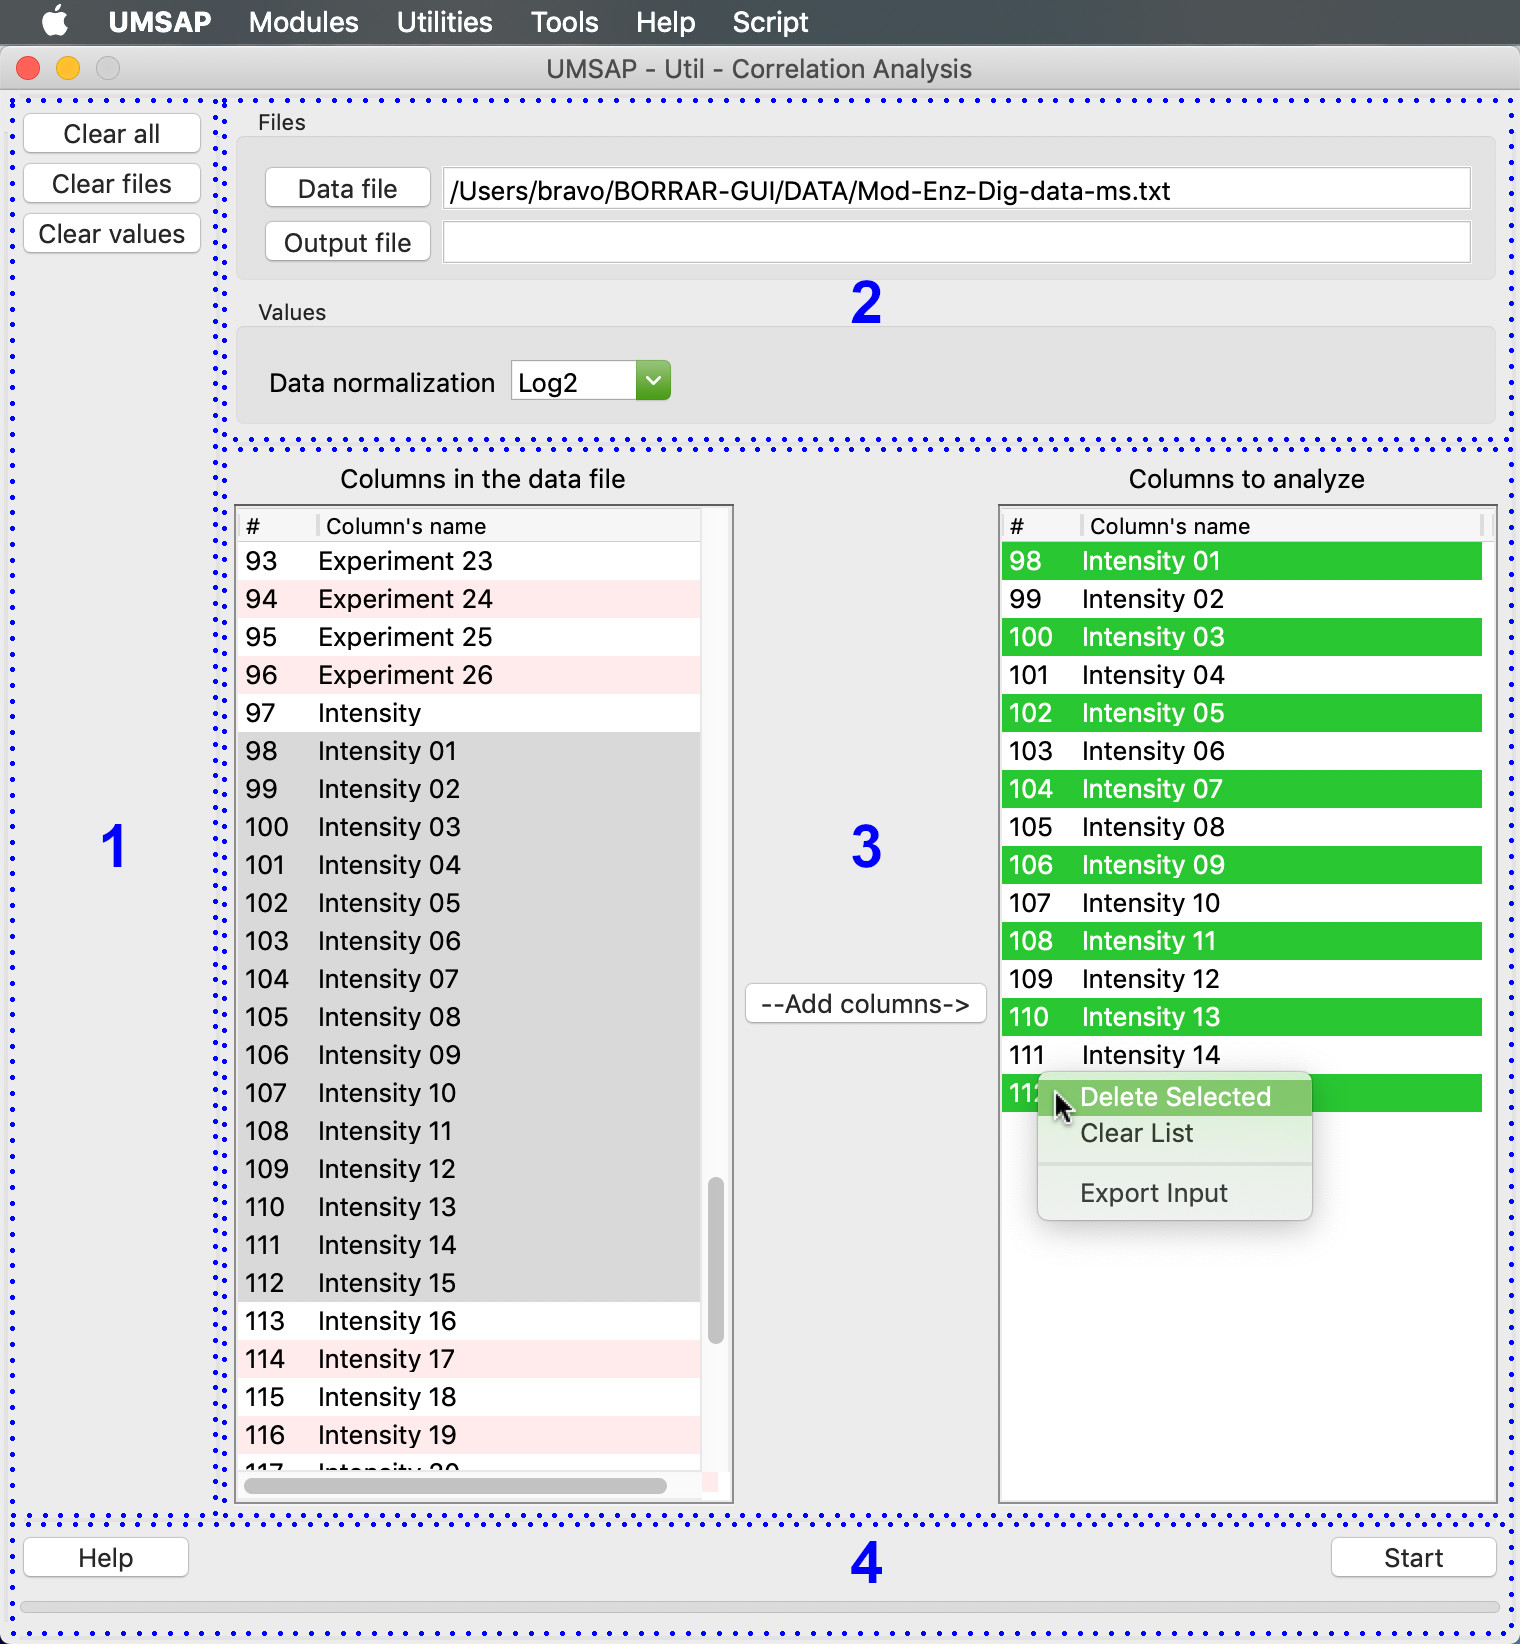
\includegraphics[width=0.7\textwidth]{./IMAGES/UTIL-CORR-WINDOW/util-corr.jpg}	    
	\caption[The Correlation Analysis utility window]{\textbf{The Correlation Analysis utility window.} This windows allows to perform a correlation analysis of the data contained in a given Data file.} 
	\label{fig:utilCorrAnalysis}
	\vspace{-5pt} 	
\end{figure}

The list box to the right of Region \num{3} contains the columns for which the correlation analysis will be performed. Correlation between all columns in the right list box will be performed. The  order of the rows and columns in the resulting matrix containing the correlation coefficients will be the same as the order of the columns shown in the right list box. Therefore, users are advised to fill the right list box in such a way that replicates of the same experiment are consecutive to each other in the right list box. Columns in the right list box can be deleted by selecting the columns and then using the right mouse button over the right list box or using the Tools menu. Columns in the right list box will be unique, meaning that a column can only be added once. 

Region \num{4} contains the Help and Start analysis buttons and a progress bar. The Help button leads to an online tutorial while the Start analysis button will start the analysis. The progress bar will give users a rough idea of the remaining processing time once the analysis is started.

\begin{figure}[h]
	\centering
	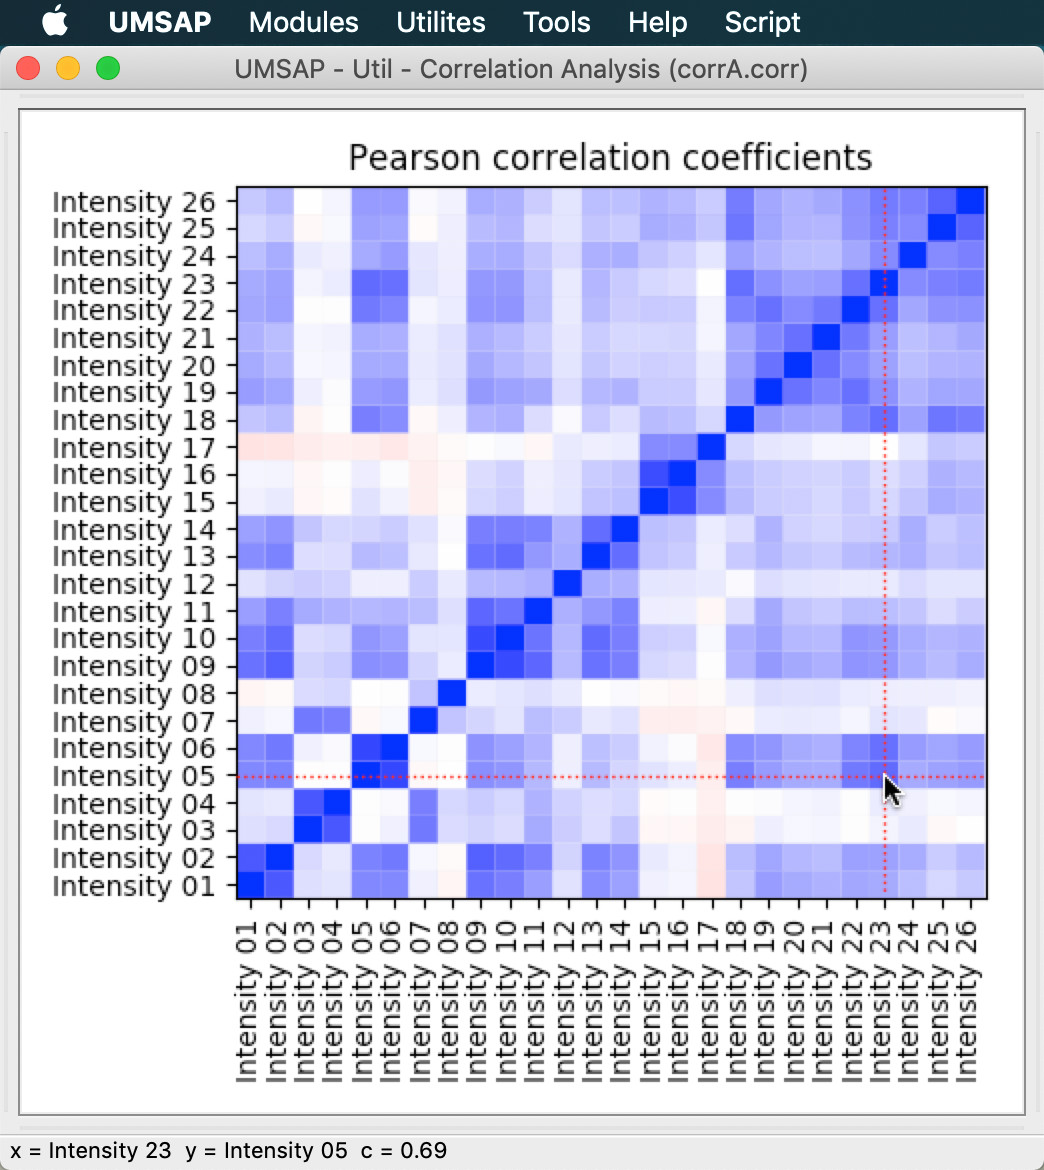
\includegraphics[width=0.7\textwidth]{./IMAGES/UTIL-CORR-WINDOW/util-corr-res.jpg}	    
	\caption[The Correlation Analysis result window]{\textbf{The Correlation Analysis result window.} The correlation coefficients are shown in a color coded matrix. Values between \numrange{-1}{0} are shown in shades of red, \num{0} is shown in white and values between \numrange{0}{1} in shades of blue. NA values are shown in green.}
	\label{fig:utilCorrAnalysisRes}
	\vspace{-5pt} 	
\end{figure} 

\textit{\textbf{The analysis}}

First, UMSAP will check the validity of the user provided input. Then, columns in the right list box are read from the Data file. The columns must contain only numbers and the same amount of rows must be found in all columns. Failing to comply with this will result in the program aborting the analysis. After this, the selected normalization procedure is applied to the data. Finally, the correlation coefficients are calculated using the selected method. If any of the coefficients cannot be calculated, then the corresponding coefficient is set to NA. After the analysis is done the results will be automatically loaded and displayed in a new window, see \autoref{fig:utilCorrAnalysisRes}. 

\textit{\textbf{The output}}

The extension .corr is reserved for a file containing the output from a correlation analysis. The results in a .corr file will be shown as a color coded matrix, see \autoref{fig:utilCorrAnalysisRes}. Values between \numrange{-1}{0} will be shown in shades of red, \num{0} will be shown as white and values between \numrange{0}{1} will be shown in shades of blue. NA values will be shown in green. The columns and rows of the matrix are the column numbers used to calculate the correlation. Information about a specific matrix element can be obtain by simply putting the mouse pointer over the matrix element.  

\textit{\textbf{The Tools menu}}

The Tools menu in the configuration window of the correlation analysis, see \autoref{fig:utilCorrAnalysis} allows users to empty the right list box or to remove only the selected rows.

The Tools menu in the window showing the results in a .corr file, see \autoref{fig:utilCorrAnalysisRes} allows user to create an image of the plot and to export the results to one of the modules in UMSAP. After selecting to export the data, the same window used to configure the Results - Control Experiment for the selected module will appear allowing users to configure this parameter and send the configuration to the module window. The exported information includes the path to the Data file used to calculate the correlation coefficients.

\subsection{Create Input File}
\label{subsec:utilUscrFile}

The Create Input File utility allows user to read a .limprot, .protprof or .tarprot file to create a .uscr file. How to generate the .limprot, .protprof or .tarprot file is discussed in \autoref{chap:limprot}, \autoref{chap:protprof} and \autoref{chap:tarprot} respectively. The .uscr file is used to prepare a module to perform an analysis without users having to type in all the information required by the module. Thus, if a second analysis of a Data file is needed users can quickly load the .uscr file into UMSAP, apply the required modifications in the window of the module and start the analysis without having to type in or modify the options that will be the same between the old and new analysis. Each .uscr file can contain information for configuring one module and one analysis.

\textit{\textbf{The interface}}

The Create Input File utility does not have a window since there are no options to specify. When the utility is selected users will be asked to select the .limprot, .protprof or .tarprot file and then users must select the output file. That is all.

\textit{\textbf{The analysis}}

First, UMSAP will check the validity of the user provided input. Then the .limprot, .protprof or .tarprot file will be read in and the configuration values will be extracted and saved in the .uscr file. The utility is able to process .tarprot files from previous versions of UMSAP.

\textit{\textbf{The output}}

The .uscr file has a simple format in which each line has a keyword and an argument. The keyword and the argument are separated by a colon (:). The following are examples of the format of the .uscr file for ech module.\newline

\textit{Example for the Limited Proteolysis module:}

Module: Limited Proteolysis\newline
Data file: /Users/kenny/data-kbr.txt\newline
Sequence (rec): /Users/kenny/seqA.txt\newline
Sequence (nat): /Users/kenny/seqA-nat.txt\newline
Output folder: /Users/kenny/test\newline
Output name: myLimTest\newline
Target protein: Mis18alpha\newline
Score value: 10\newline
Sequence length: 100\newline
d-value: NA\newline
dm-value: 8\newline
Data normalization: Log2\newline
a-value: 0.050\newline
b-value: Equal alpha\newline
y-value: 0.8\newline
Sequence: 0\newline
Detected proteins: 34\newline
Score: 42\newline
Columns to extract: 0 1 2 3 4-10\newline
Results: 69-71; 81-83, 78-80, 75-77, 72-74, NA; NA, NA, NA, 66-68, NA; 63-65, 105-107, 102-104, 99-101, NA; 93-95, 90-92, 87-89, 84-86, 60-62\newline

\textit{Example for the Proteome Profiling module:}

Module: Proteome Profiling\newline
Data file: /Users/kenny/proteinGroups-kbr.txt\newline
Output folder: /Users/kenny/test\newline
Output name: myProtTest\newline
Score value: 320\newline
Z score: 10\newline
Data normalization: Log2\newline
a-value: 0.050\newline
Median correction: True\newline
P correction: Benjamini - Hochberg\newline
Detected proteins: 0\newline
Gene names: 6\newline
Score: 39\newline
Exclude proteins: 171 172 173\newline
Columns to extract: 0 1 2 3 4-10\newline
Results: 105 115 125, 130 131 132; 106 116 126, 101 111 121; 108 118 128, 103 113 123\newline
Conditions: DMSO, H2O\newline
Relevant Points: 30min, 1D\newline
Control Type: One Control per Column\newline
Control Label: MyControl\newline

\textit{Example for the Targeted Proteolysis module:}

Module: Targeted Proteolysis\newline
Data file: /Users/kenny/data-ms.txt\newline
Sequence (rec): /Users/kenny/data-seq.txt\newline
Sequence (nat): P31545\newline
PDB file: NA\newline
Output folder: /Users/kenny/test\newline
Output name: myTarTest\newline
Target protein: efeB\newline
Score value: 200\newline
Data normalization: Log2\newline
a-value: 0.050\newline
Positions: 5\newline
Sequence length: 100\newline
Histogram windows: 50\newline
PDB ID: 2y4f;A\newline
Sequence: 100\newline
Detected proteins: 38\newline
Score: 44\newline
Columns to extract: 0 1 2 3 4-10\newline
Results: 98-105; 109-111; 112 113 114; 115-117 120\newline

The menu entry Run Input File in the Script menu allows to load the .uscr file into UMSAP.

\subsection{Merge aadist Files}
\label{subsec:utilMergeAadistFiles}

The .aadist files contain an AA distribution analysis as described in \autoref{subsec:utilAadistCalc}. The Merge aadist Files utility allows to merge several .aadist files into a single file.

\textit{\textbf{The interface}}

The Merge aadist Files window is divided in four regions, see \autoref{fig:utilMergeAadist}.

\begin{figure}[h]
	\centering
	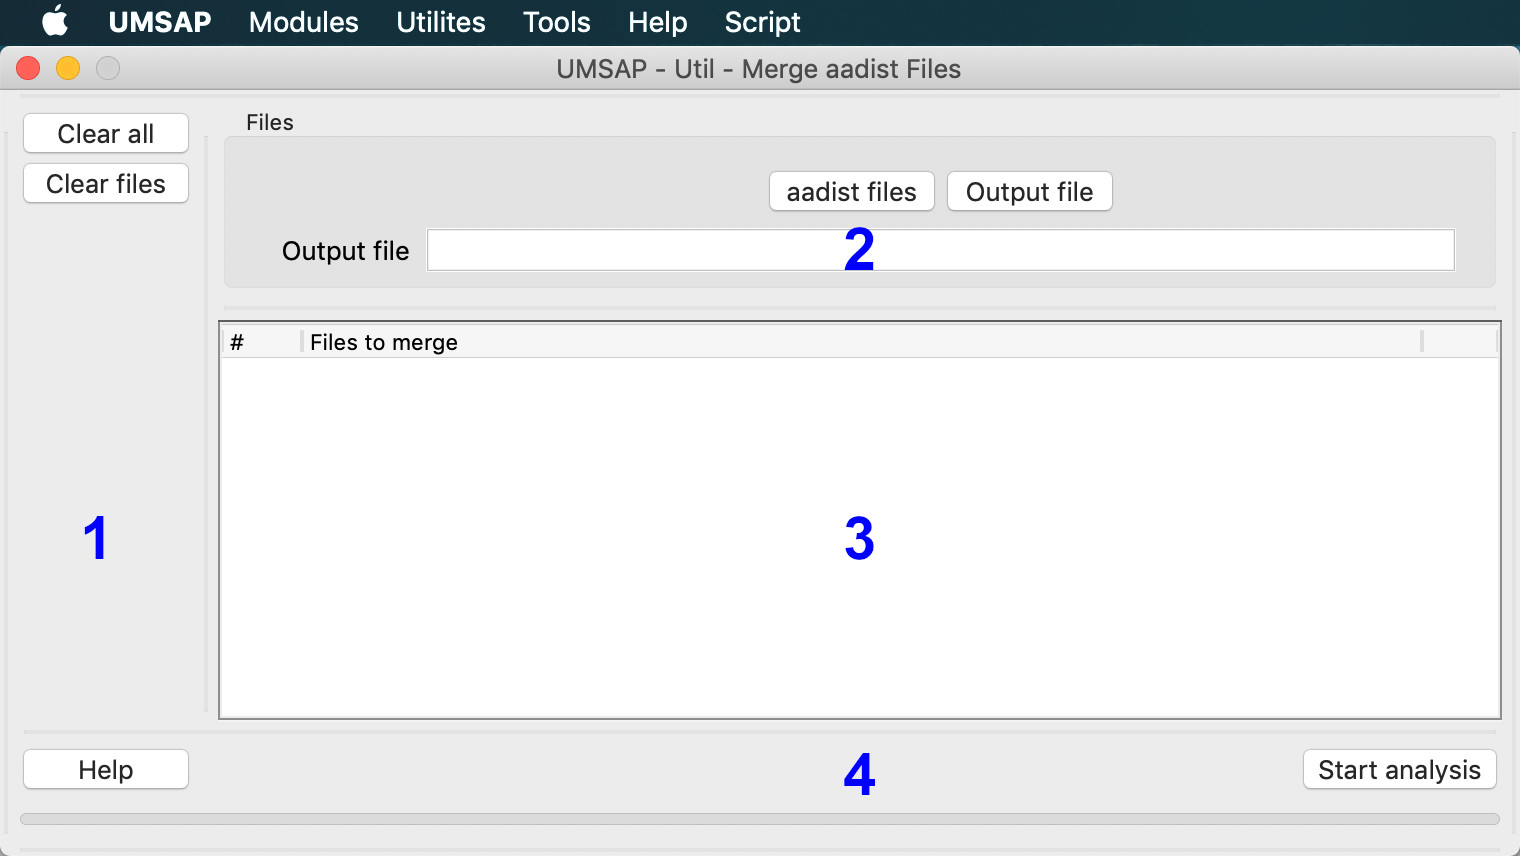
\includegraphics[width=0.7\textwidth]{./IMAGES/UTIL-Maadist-WINDOW/util-maadist.jpg}	    
	\caption[The Merge .aadist Files utility window]{\textbf{The Merge .aadist Files utility window.} This window allows users to merge several .aadist files in a single file.}
	\label{fig:utilMergeAadist}
	\vspace{-5pt} 	
\end{figure}

Region \num{1} contains two buttons allowing users to quickly delete all provided input and start a new calculation. The Clear all button will delete all user provided input and will reset the state of the list box in Region \num{3}. The Clear files button will reset the state of the list box in Region \num{3} and delete all user provided paths to files.

Region \num{2} contains the fields where users provide the information needed in order to merge the .aadist files. The aadist files button allows users to browse the file system to select multiple .aadist file from a folder. Only .aadist files can be selected here. Once the files are selected the complete path to the files will be displayed in the list box in Region \num{3}. The Output file button allows users to browse the file system to select the location and name of the output file.

Region \num{3} contains a list box showing all selected .aadist files. Files can only be added one time to the list box. The order of the files in the list box is meaningless. Selected files can be deleted from the list box by pressing the right mouse button over the list box or using the Tools menu. 

Region \num{4} contains the Help and Start analysis buttons and a progress bar. The Help button leads to an online tutorial while the Start analysis button will start the analysis. The progress bar will give users a rough idea of the remaining processing time once the analysis is started.

\textit{\textbf{The analysis}}

First, UMSAP will check the validity of the user provided input. Then, the number of positions and experiments in each .aadist files are checked. If they do not match, the merging is aborted. Finally, UMSAP check that all AA distributions were originated from the same sequence and abort the task at hand if they do not. After this, files are merged. For merging the files, UMSAP adds the number of times each amino acids appears in a given position for each file. Finally, UMSAP performs the $\chi^2$ test, as indicated in \autoref{subsec:utilAadistCalc}. The significance level for the merged file is the highest value found in all files that were merged. When all files have been merged the results will be automatically loaded and displayed in a new window, see \autoref{fig:utilAadistShow}. 

\textit{\textbf{The output}} 

The Merge aadist Files utility generates a .aadist file. This file can be visualized in the same way as the output from the AA distribution utility, see \autoref{subsec:utilAadistCalc} for more details.

\subsection{Read Output File}
\label{subsec:utilReadOutF}

The Read Output File utility simply loads an output file generated by UMSAP. After selecting this option from the Utility window (\autoref{fig:utilWindow}) or the Utilities menu entry, a dialog box will be presented allowing users to select some of the output files generated by UMSAP. Currently, only .aadist, .corr, .cutprop, .hist, .limprot, .protprof, and .tarprot files can be selected. After selecting the file, the appropriate window showing the graphical representation of the file will be created. 

\subsection{Run Input File}
\label{subsec:utilReadUscr}

The Run Input File utility allows to load a .uscr file and launches the appropriate module. The information found in the selected .uscr file is used to fill the interface of the module. Incorrect keywords - value pairs in the .uscr are silently ignored. This utility does not have an interface since the only thing required is users to select a .uscr file.

\subsection{Short Data Files}
\label{subsec:utilShortDF}

The Short Data Files utilities allows users to create short versions of the Data file used to create a .limprot, .protprof or .tarprot file. How to generate the .limprot, .protprof or .tarprot file is discussed in \autoref{chap:limprot}, \autoref{chap:protprof} and \autoref{chap:tarprot} respectively.

\textit{\textbf{The interface}}

The Short Data Files window is divided in three regions, see \autoref{fig:utilShortData}.

\begin{figure}[h]
	\centering
	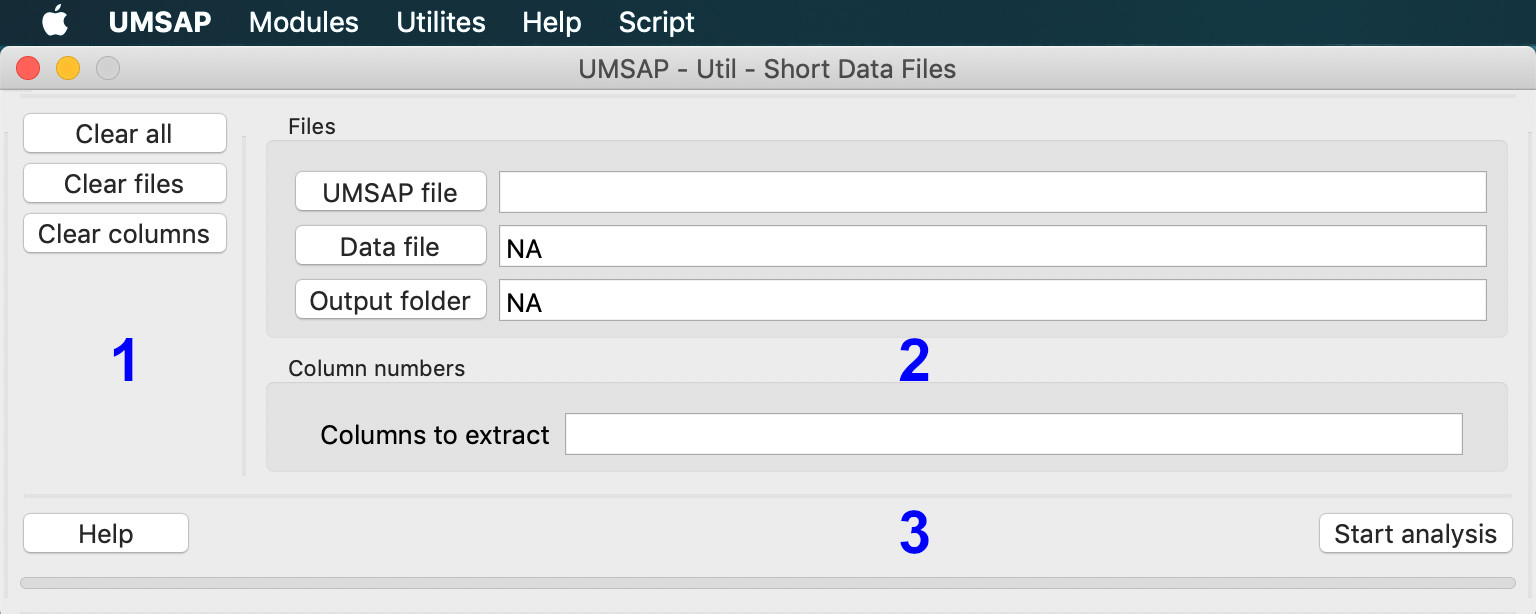
\includegraphics[width=0.7\textwidth]{./IMAGES/UTIL-SHORTDF-WINDOW/util-shortdf.jpg}	    
	\caption[The Short Data File utility window]{\textbf{The Short Data File utility window.} This window allows to generate smaller versions of the Data file used to generate a .limport, .protprof or a .tarprot file.} 
	\label{fig:utilShortData}
	\vspace{-5pt} 	
\end{figure} 

Region \num{1} contains three buttons allowing user to quickly delete all provided input and start a new analysis. The Clear all button will delete all user provided input. The Clear files button will delete the path to all user provided files. Finally, the Clear values button will delete all user provided numerical values.

Region \num{2} contains the fields where users provide the information needed in order to generate the short data files. The UMSAP file button allows users to browse the file system to select the .limprot, .protprof or .tarprot file that will be used for the analysis. Only one file can be provided here. The Data file button allows users to browse the file system to select the Data file that will be used for the analysis. The Short Data File utility generates multiple files that will be saved in a folder named Data. The Output folder button allows users to browse the file system to select a location for the output folder Data. If the Output folder option is left empty, the output folder Data will be created in the same directory as the UMSAP file. If there is a Data folder in the selected Output folder, then UMSAP will create a new Data folder with the date and time to the second added to the end of the name in order to avoid overwriting any file. 

The parameter Columns to extract allows to define which columns from the data file will be extracted to the short data files. The values here are expected to be integers greater than zero.

Region \num{3} contains the Help and Start analysis buttons and a progress bar. The Help button leads to an online tutorial while the Start analysis button will start the analysis. The progress bar will give users a rough idea of the remaining processing time once the analysis is started.

\textit{\textbf{The analysis}}

First, UMSAP will check the validity of the user provided input. If only an UMSAP file is given, then the data file location will be read from the UMSAP file. After this, the short data files will be written to the Data folder.

\textit{\textbf{The output}}

For the Limited Proteolysis and Targeted Proteolysis modules the output consist of three files that will be saved in a Data folder. Assuming that the name of the Target protein is efeB, the name of the files will be:\newline 
all-columns-all-efeB-records.txt \newline
selected-columns-all-efeB-records.txt \newline
selected-columns-relevant-efeB-records.txt

These files are just shorter versions of the Data file containing only relevant information about the Target protein. They are plain text files with a tabular format. The first row contains the name of the columns and columns are tab separated. The file all-columns-all-efeB-records.txt contains the same number of columns as the Data file but only the rows for the Target protein. The file selected-columns-all-efeB-records.txt contains only rows for the Target protein and the columns specified in Columns to extract. The selected-columns-relevant-efeB-records.txt file is similar to the previous file but contains only the relevant peptides of the Target protein. 

In the case of the Proteome Profiling module only one file is generated. The file contains all the rows in the Data file but only the selected columns.

In all cases, these files can be viewed with any text editor.





